\documentclass{beamer}

\newcommand\tab[1][1cm]{\hspace*{#1}}
\usepackage[spanish]{babel}
\usepackage[utf8]{inputenc}
\usepackage{bussproofs}
\usepackage{url}
\usepackage[document]{ragged2e}
\usepackage{tikz}
\usetikzlibrary{shapes,arrows,spy,positioning,snakes}
\usepackage{verbatim} % comentarios
\usepackage{tabulary} % tablas

\DeclareOptionBeamer{compress}{\beamer@compresstrue}
\ProcessOptionsBeamer

\mode<presentation>

\useoutertheme[footline=authortitle]{miniframes}
\useoutertheme{infolines}
\useinnertheme{circles}
\usecolortheme{whale}
\usecolortheme{orchid}

\definecolor{beamer@blendedblue}{rgb}{0.137,0.466,0.741}

\setbeamercolor{structure}{fg=beamer@blendedblue}
\setbeamercolor{titlelike}{parent=structure}
\setbeamercolor{frametitle}{fg=black}
\setbeamercolor{title}{fg=black}
\setbeamercolor{item}{fg=black}

\setbeamertemplate{bibliography item}[text]

\mode
<all>

\title[]{Introducción a Hyperledger Fabric}
\subtitle{Fundamentos de blockchains}
\author{René Dávila - Jorge Solano}
%\institute{IIMAS}
\date{ }

\AtBeginSection[] { 
	\begin{frame} 
		\frametitle{Índice}
		\tableofcontents[currentsection]
	\end{frame}
}
\AtBeginSubsection[] { 
	\begin{frame}
		\frametitle{Índice}
		\tableofcontents[currentsection, currentsubsection]
	\end{frame}
}

\setbeamertemplate{navigation symbols}{}

\begin{document}
	\EnableBpAbbreviations
	
	\begin{frame}
		\begin{center}
			
\includegraphics [width =0.2 \textwidth ]{iimas}
		\end{center}
		\titlepage 
	\end{frame}

%\begin{comment}
	\section{Introducción}
	\begin{frame}
		\begin{block}{Hyperledger project}
			La Linux Foundation se caracteriza por nutrir proyectos \textbf{open source} de \textbf{open governance} que genera comunidades sostenibles fuertes y ecosistemas prósperos.\\
			\vspace{4mm}
			\textbf{Linux Foundation} creó el projecto \textbf{Hyperledger} en 2015 para avanzar en la industria de la tecnología de blockchain.
		\end{block}
	\end{frame}

	\begin{frame}
		\begin{block}{Hyperledger project}
			\textbf{Hiperledger Fabric} es uno de los \textbf{proyectos de blockchain en Hyperledger}, el cual es un ledger que utiliza smart contracts y donde los participantes manejan las transacciones.
		\end{block}
	\end{frame}

	\subsection{Blockchain}
	\begin{frame}
		\frametitle{Blockchain}
		En términos generales, una \textbf{blockchain} se podría considerar como un \textbf{libro mayor} en el área contable \textbf{(ledger)}. Es un lugar donde se llevan a cabo transacciones inmutables dentro de una red de nodos distribuida.\\
		\vspace{4mm}
		Cada uno de estos \textbf{nodos} mantiene una \textbf{copia del libro mayor} aplicando transacciones que han sido validadas mediante el protocolo de consenso, agrupadas en bloques que incluyen un hash que permite enlazar cada bloque con su bloque anterior.
	\end{frame}
	
	\subsection{Criptomonedas}
	\begin{frame}
		\frametitle{Criptomonedas}
		La aplicación más reconocida de blockchain es la criptomoneda \textbf{Bitcoin}.\\
		\vspace{4mm}
		\textbf{Ethereum} es una criptomoneda alternativa, la cual integra muchas características de Bitcoin, pero agrega contratos inteligentes (smart contracts) con el fin de crear una plataforma para aplicaciones distribuidas.
	\end{frame}
	
	\begin{frame}
		Tanto \textbf{Bitcoin} como \textbf{Ethereum} caen en la clasificación de blockchain, las cuales clasificaremos como tecnologías de \textbf{blockchain públicas y sin permiso}. Básicamente, son redes públicas, abiertas a cualquiera, donde los participantes interactúan de manera anónima.
	\end{frame}

	\begin{frame}
		Sin embargo, en muchos casos de \textbf{uso empresarial} la \textbf{identidad} de los participantes es un \textbf{requisito indispensable}, como por ejemplo en una transacción financiera, donde las regulaciones el Know Your Customer (KYC) y el Anti-Money Laundering (AML) deben seguirse de manera puntual.
	\end{frame}
	
	\begin{frame}
		Para el uso empresarial de blockchain se deben considerar los siguientes requerimientos:
		
		\begin{itemize}
			\item Cada participante debe identificarse y ser identificable.
			\item Las redes deben estar autorizadas.
			\item Alto rendimiento durante las transacciones.
			\item Baja latencia en la confirmación de transacción.
			\item Privacidad y confidencialidad de las transacciones y de la información de las transacciones.
		\end{itemize}
	\end{frame}
	
	\section{Hyperledger Fabric v2.0}
	
	\begin{frame}
		\begin{block}{Hyperledger Fabric v2.0}
			Hyperledger Fabric es una plataforma \textbf{open source} de grado \textbf{empresarial}, que permite manejar un tecnología distribuida de ledger (una blockchain).\\
			\vspace{4mm}
			Tiene algunas \textbf{capacidades claves} diferentes con respecto a otros ledger distribuidos o a otras plataformas de blockchain.
		\end{block}
	\end{frame}

	\subsection{Componentes y características}
	
	\begin{frame}
		\frametitle{Private and permissioned}
		\textbf{Hiperledger Fabric} destaca por sobre otros sistemas de blockchain porque \textbf{es privada y autorizada}, esto es, los miembros de la red se registran a través de un Membership Service Provider (MSP) de confianza.\\
	\end{frame}

	\begin{frame}
		Entonces, por ejemplo, si los participantes no pueden confiar completamente uno en el otro (por ejemplo, si son competidores en la misma industria), la red puede operar bajo el modelo de \textbf{gobierno  basado en la confianza} que existe entre los participantes, como lo es un acuerdo legal o un marco de referencia para manejar disputas.
	\end{frame}
	
	\begin{frame}
		\frametitle{Pluggable}
		\textbf{Hyperledger Fabric} ofrece varias \textbf{opciones enchufables}. La información del ledger puede guardarse en múltiples formatos, los mecanismos de consenso se pueden intercambiar y se pueden tener diferentes Provedores de Servicio de Membresía (MSP).\\
		\vspace{4mm}
		Esto permite que la plataforma sea \textbf{personalizada} y se ajuste a casos de uso y modelos confiables particulares.
	\end{frame}

	\begin{frame}	
		Por ejemplo, dentro de una empresa o en una empresa operada por una autoridad de confianza, el protocolo de consenso tolerante a fallas bizantinas podría considerarse innecesario y hasta excesivo, en su lugar se podría pensar que el \textbf{protocolo de consenso tolerante a fallas} sería más apropiado.
	\end{frame}
	
	\begin{frame}
		\frametitle{Channels}
		\textbf{Hyperledger Fabric} ofrece la posibilidad de crear \textbf{canales}, lo que permite que un grupo de participantes tenga su propio ledger de transacciones.\\
		\vspace{4mm}
		Esta capacidad es importante en redes donde algunos participantes pueden ser competidores y no quieren que cada transacción (pe, una oferta especial en un producto) sea conocida por cada participante.
	\end{frame}

	\begin{frame}
		\frametitle{Shared Ledger}
		El ledger de \textbf{Hyperledger Fabric} comprende dos componentes: el \textbf{world state} y la \textbf{transaction log}. Cada participante tiene una copia del ledger de cada red a la que pertenece.\\
		\vspace{4mm}
		El world state representa la base de datos del ledger. La transaction log guarda la historia actualizada del world state. El ledger es, entonces, la combinación de la \textbf{BD} del world state y la historia de la \textbf{transaction log}.
	\end{frame}
	
	\begin{frame}
		\frametitle{Smart contracts}
		Los \textbf{smart contracts} de \textbf{Hyperledger Fabric} están escritos en chaincode y son invocados por una aplicación externa a la blockchain. En la mayoría de los casos, el chaincode interactúa directamente con la base de datos del ledger (world state) y no con la log transaction.\\
		\vspace{4mm}
		El \textbf{chaincode} puede ser implementado \textbf{en lenguajes de programación de uso general} (como Java, Go y Node.js), por lo que no se requiere aprender un lenguaje de dominio específico.\\
	\end{frame}

	\begin{frame}
		\frametitle{Privacy}
		\textbf{Hyperledger Fabric} permite crear tanto redes donde la \textbf{privacidad} (utilizando canales) es un requerimiento operacional clave, así como redes abiertas.
	\end{frame}
	
	\begin{frame}
		\frametitle{Consensus}
		\textbf{Hyperledger Fabric} está diseñado para permitir que las redes elijan el \textbf{mecanismo de consenso} que mejor se acomode a la relación que existe entre los participantes.
	\end{frame}
		
	\begin{frame}
		\textbf{Fabric} puede aprovechar los protocolos de consenso que \textbf{no requieren criptomonedas} nativas para incentivar la minería o la ejecución de contratos inteligentes. Evitar las criptomonedas \textbf{reduce} de manera significativa \textbf{el riesgo o los vectores de ataque}.\\
		\vspace{4mm}
		Además, la ausencia de las operaciones de minería criptográfica permite que la plataforma se pueda desplegar con prácticamente el mismo costo operacional que cualquier otro sistema distribuido. 
	\end{frame}
	
	\section{Instalación de Hyperledger Fabric v2.0}
	
	\begin{frame}
		Para poder ejecutar los proyectos de \textbf{Hyperledger Fabric} es necesario tener ciertas herramientas ya instaladas. Entonces, primero hay que verificar o instalar los \textbf{prerrequisitos de instalación}.
	\end{frame}
	
	\subsection{Prerrequisitos de instalación}
	
	\begin{frame}
		\frametitle{Prerrequisitos de instalación}
		Para poder desarrollar aplicaciones con Hyperledger Fabric se deben tener instaladas las siguientes herramientas:
		\begin{itemize}
			\item Git
			\item curl
			\item Docker y Docker Compose (versión 17.06.2-ce o superior)
			\item Go
			\item Node.js y NPM
			\item Python
		\end{itemize}
	\end{frame}
	
	\begin{frame}
		\frametitle{Git (\url{https://git-scm.com/downloads})}
		\textbf{Git} es un \textbf{controlador de versiones distribuido}, gratuito y de código abierto diseñado para manerjar proyectos de diferente tamaño con eficiencia.
		\begin{figure}[h]
			
\includegraphics[scale=.3]{git}
			\centering
		\end{figure}
	\end{frame}

	\begin{frame}
		\frametitle{curl (\url{https://curl.haxx.se/download.html})}
		\textbf{curl} (Client URL) es una biblioteca y una herramienta de línea de comandos que permite \textbf{transferir datos} a través de diferentes protocolos.
		\begin{figure}[h]
			
\includegraphics[scale=.3]{curl}
			\centering
		\end{figure}
	\end{frame}

	\begin{frame}
		\frametitle{Docker (\url{https://www.docker.com/get-docker})}
		\textbf{Docker} es un \textbf{contenedor de aplicaciones}. Un contenedor es una unidad estándar de software que empaqueta código y todas sus dependencias para que la aplicación se ejecute de manera confiable y rápida en cualquier entorno de computadora.
		\begin{figure}[h]
			
\includegraphics[scale=.3]{docker}
			\centering
		\end{figure}
	\end{frame}
	
	\begin{frame}
		\frametitle{Docker Compose (\url{https://docs.docker.com/compose/install/})}
		\textbf{Compose} es una herramienta para definir y \textbf{ejecutar múltiples contenedores de aplicaciones} Docker. Docker-compose ya está incluida en Docker Desktop.
		\begin{figure}[h]
			
\includegraphics[scale=.3]{docker}
			\centering
		\end{figure}
	\end{frame}

	\begin{frame}
		\frametitle{Go (\url{https://golang.org/dl/})}
		\textbf{Go} es un \textbf{lenguaje de programación} de código abierto que permite crear software simple, confiable y eficiente.
		\begin{figure}[h]
			
\includegraphics[scale=.3]{go}
			\centering
		\end{figure}
	\end{frame}
	
	\begin{frame}
		\frametitle{Node.js (\url{https://nodejs.org/en/download/})}
		\textbf{Node.js} es un \textbf{entorno de ejecución de JavaScript}, de código abierto y multiplataforma, que permite ejecutar código JavaScript fuera de un navegador web.
		\begin{figure}[h]
			
\includegraphics[scale=.3]{nodejs}
			\centering
		\end{figure}
	\end{frame}
	
	\begin{frame}
		\frametitle{NPM (\url{https://www.npmjs.com/get-npm})}
		\textbf{NPM} es un \textbf{administrador de paquetes} para el lenguaje de programación JavaScript. Es el administrador de paquetes por defecto de Node.js.
		\begin{figure}[h]
			
\includegraphics[scale=.3]{npm}
			\centering
		\end{figure}
	\end{frame}
	
	\begin{frame}
		\frametitle{Python (\url{https://www.python.org/downloads/})}
		\textbf{Python} \textbf{lenguaje de programación interpretado}dwcx, de alto nivel y de propósito general.
		\begin{figure}[h]
			
\includegraphics[scale=.3]{python}
			\centering
		\end{figure}
	\end{frame}

	\subsection{Instalación}
	
	\begin{frame}
		\frametitle{Instalación}
		Una vez \textbf{instalados los prerrequisitos}, se tiene el ambiente necesario para \textbf{descargar e instalar Hyperledger Fabric}. Actualmente el proyecto no cuenta con un instalador de los binarios de Fabric, pero los ejemplos que se descargan poseen scripts de ejecución.
	\end{frame}
	
	\begin{frame}
		\frametitle{Instalación}
		Para la instalación simplemente hay que descargar los binarios y las imágenes de Fabric\\
		\begin{center}
			\setlength{\fboxrule}{1mm}
			\setlength{\fboxsep}{3mm}
			\framebox[9cm][c]{
					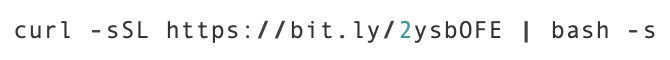
\includegraphics[scale=.7]{install_01}
			}
		\end{center}
	\end{frame}

	\begin{frame}
		\frametitle{Instalación}
		La instrucción anterior descarga y descomprime los binarios requeridos y específicos para la plataforma y los guarda en el repositorio (\textbf{fabric-samples}) dentro de la \textbf{carpeta bin}.
		\begin{figure}[h]
			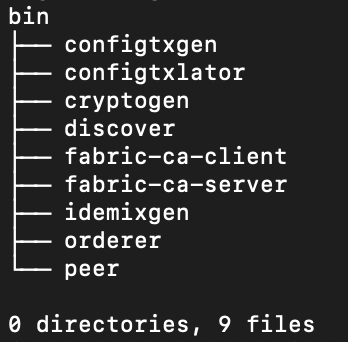
\includegraphics[scale=.5]{install_02}
			\centering
		\end{figure}
	\end{frame}
	
	\begin{frame}
		\frametitle{Instalación}
		Por último, hay que mapear la carpeta \textbf{bin al PATH} del sistema. Aquí es importante comentar que también go y go/bin deben estar en el PATH.
		\begin{center}
			\setlength{\fboxrule}{1mm}
			\setlength{\fboxsep}{3mm}
			\framebox[9cm][c]{
				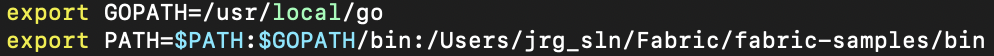
\includegraphics[scale=.5]{install_03}
			}
		\end{center}
	\end{frame}
%\end{comment}

	\section{Hyperledger en acción}
	
	\begin{frame}
		Para iniciar con la implementación de una \textbf{blockchain empresarial} (particular) se requiere tener un diagrama general de las entidades \textbf{participantes y su interacción}.\\
		\vspace{4mm}
		A continuación se describirán todos los \textbf{elementos} que pueden interactuar \textbf{en Hyperledger Fabric}, a partir de un ejemplo genérico.
	\end{frame}
	
	\subsection{Contexto}
	
	\begin{frame}
		\frametitle{Contexto}
		Se tienen 4 organizaciones (R1, R2, R3 y R4). R4 es el iniciador de la red (no hará transacciones de negocios). R1 y R2 tienen una comunicación privada en la red. De la misma manera R2 y R3.
		\begin{figure}[h]
			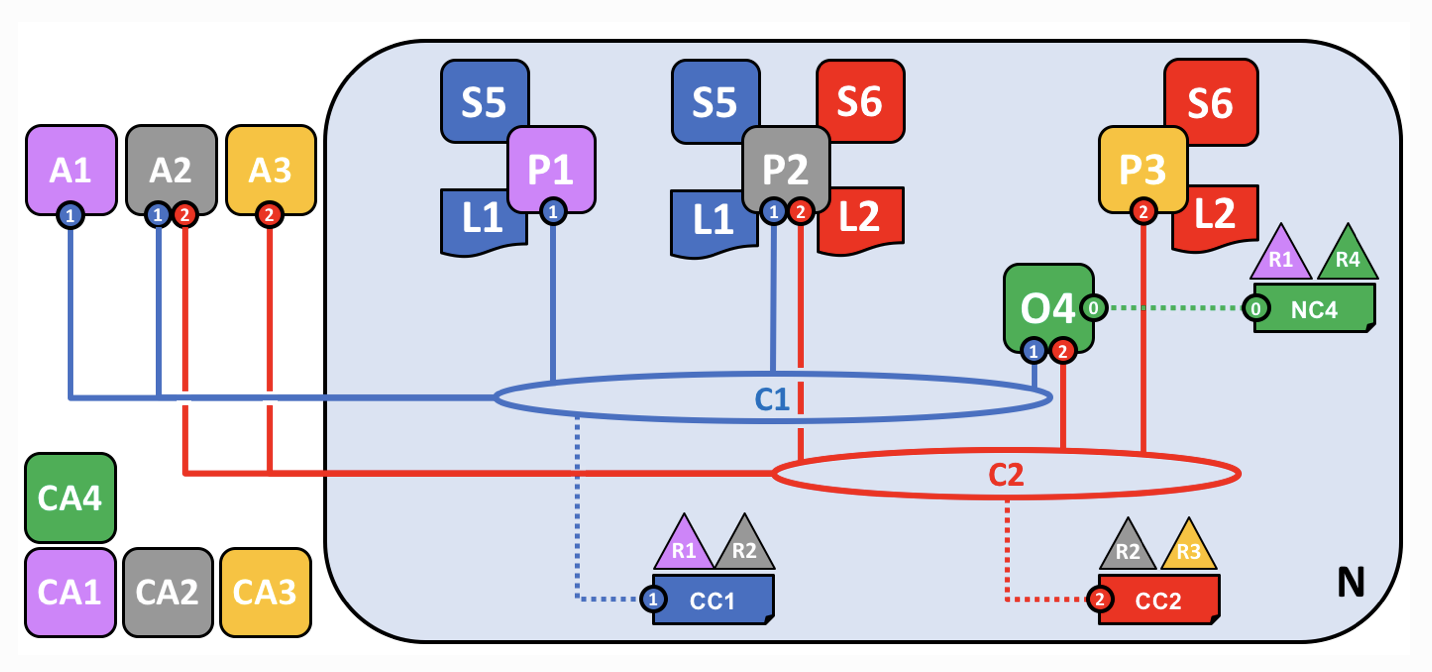
\includegraphics[scale=.3]{start_01}
			\centering
		\end{figure}
	\end{frame}
	
	\begin{frame}
		\frametitle{Contexto}
		R1 tiene una aplicación cliente A1 que hace transacciones en C1. R2 tiene una A2 que hace transacciones en C1 y en C2. R3 tiene una A3 que hace transacciones en el C2.
		\begin{figure}[h]
			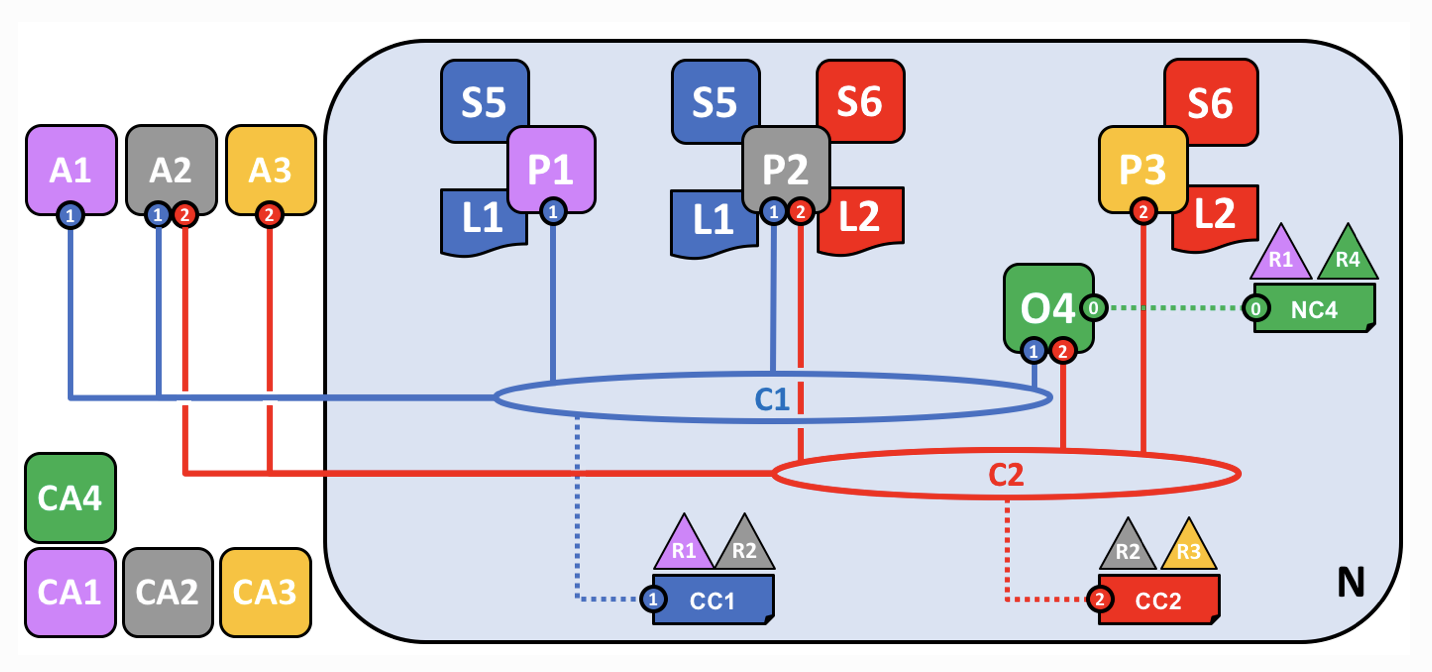
\includegraphics[scale=.3]{start_01}
			\centering
		\end{figure}
	\end{frame}
	
	\begin{frame}
		\frametitle{Contexto}
		El peer node P1 tiene una copia del ledger L1 asociado con C1 y un contrato inteligente S5. El peer node P2 tienen una copia de L1 y S5 asociado a C1 y una copia de L2 y S6 asociado a C2. El peer node P3 tiene una copia de L2 y S6 asociado a C2.
		\begin{figure}[h]
			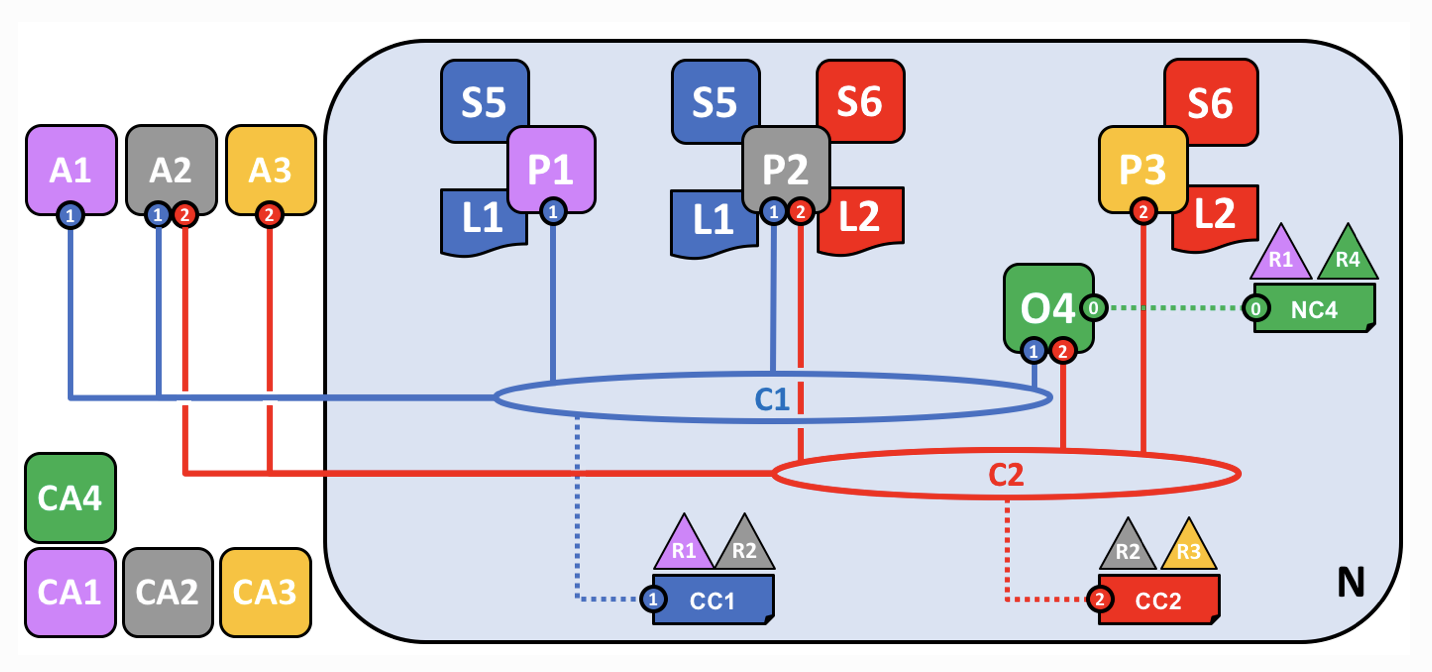
\includegraphics[scale=.3]{start_01}
			\centering
		\end{figure}
	\end{frame}
	
	\begin{frame}
		\frametitle{Contexto}
		La red está gobernada de acuerdo a las políticas especificadas en la configuración de red NC4. Las políticas están bajo el control de R1 y R4.
		\begin{figure}[h]
			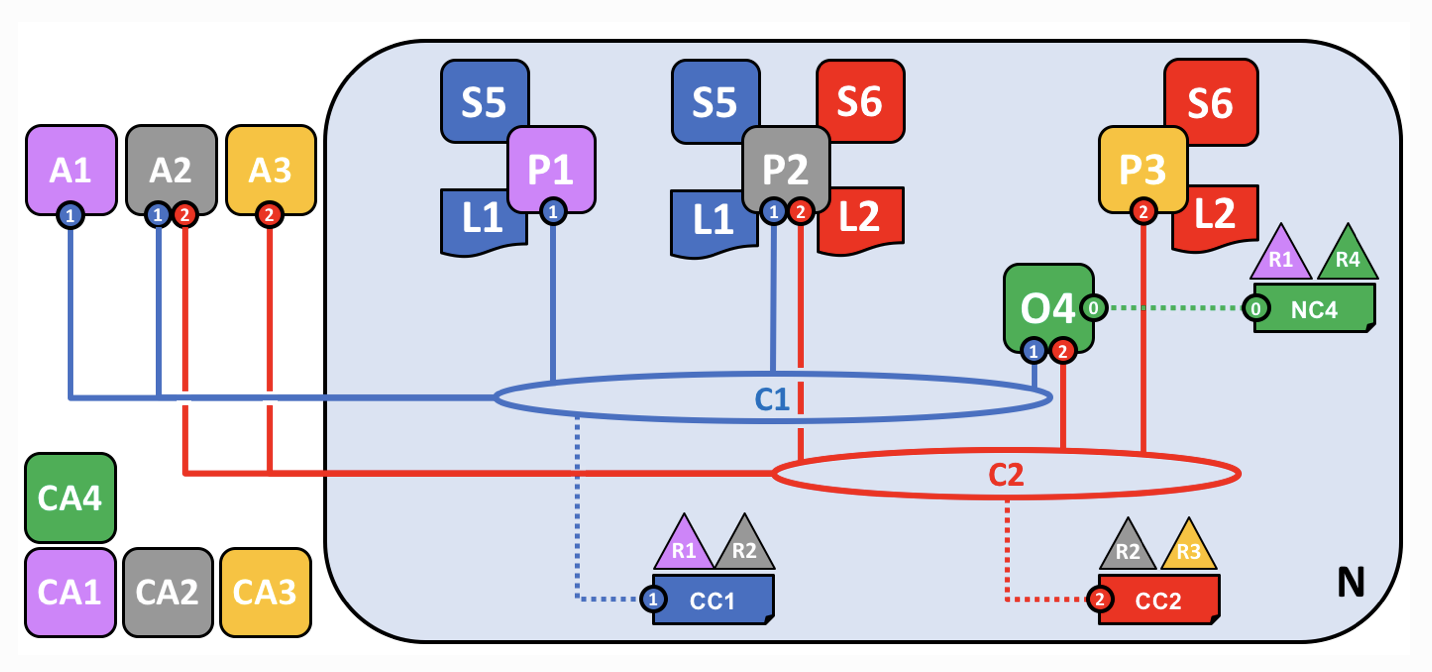
\includegraphics[scale=.3]{start_01}
			\centering
		\end{figure}
	\end{frame}

	\begin{frame}
		\frametitle{Contexto}
		C1 está gobernado de acuerdo a las políticas especificadas en la configuración del canal CC1; el canal está gobernado por R1 y R2. C2 está gobernado por las políticas especificadas en la CC2; el canal está gobernado por R2 y R3.
		\begin{figure}[h]
			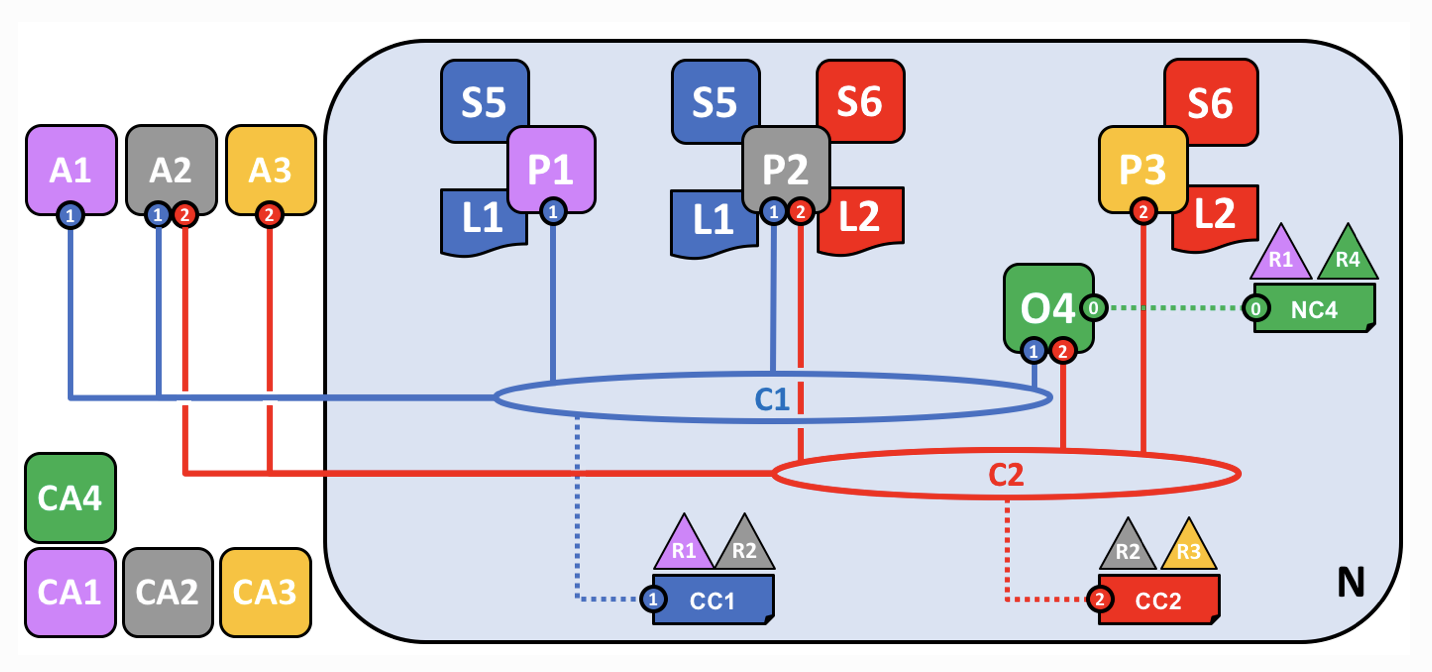
\includegraphics[scale=.3]{start_01}
			\centering
		\end{figure}
	\end{frame}

	\begin{frame}
		\frametitle{Contexto}
		Hay un nodo de ordering service O4 que funge como un punto de administración de la red N. O4 soporta los canales de aplicación C1 y C2, con el fin de ordenar los bloques de transacciones para su distrubución.
		\begin{figure}[h]
			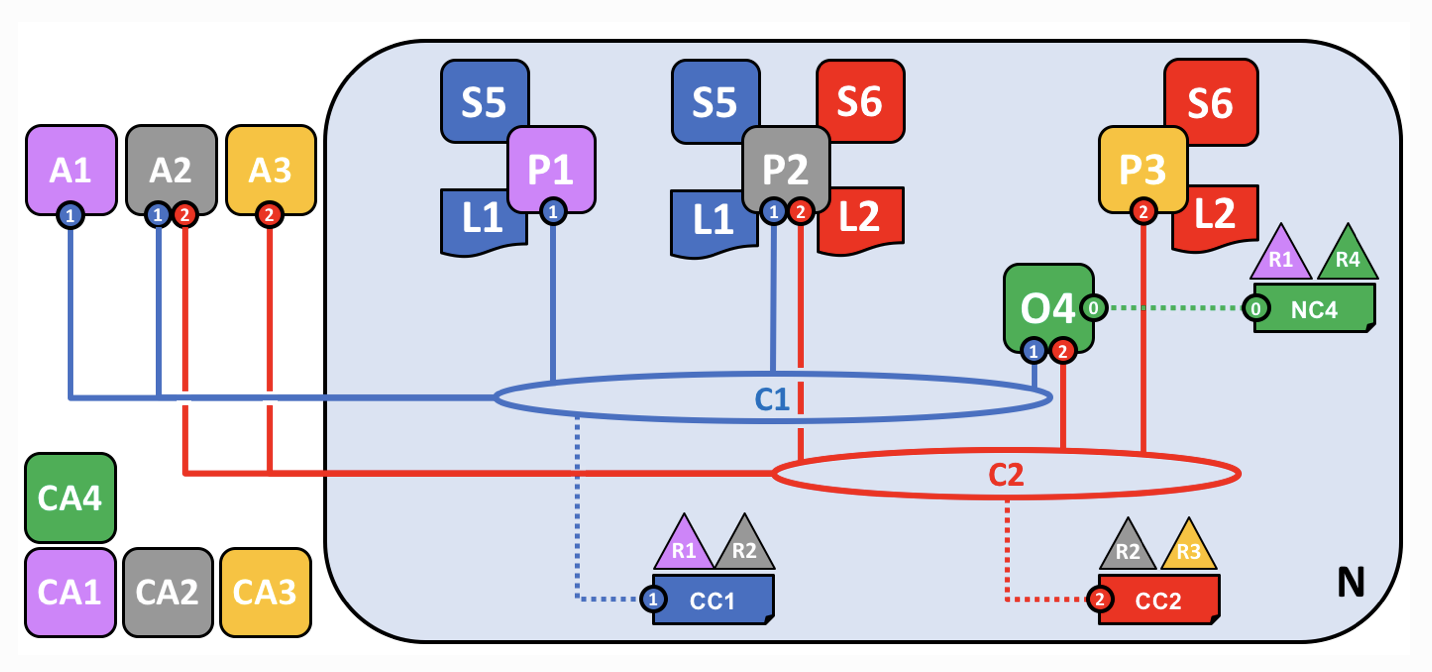
\includegraphics[scale=.3]{start_01}
			\centering
		\end{figure}
	\end{frame}

	\begin{frame}
		\frametitle{Contexto}
		Ordering sevice
		\begin{figure}[h]
			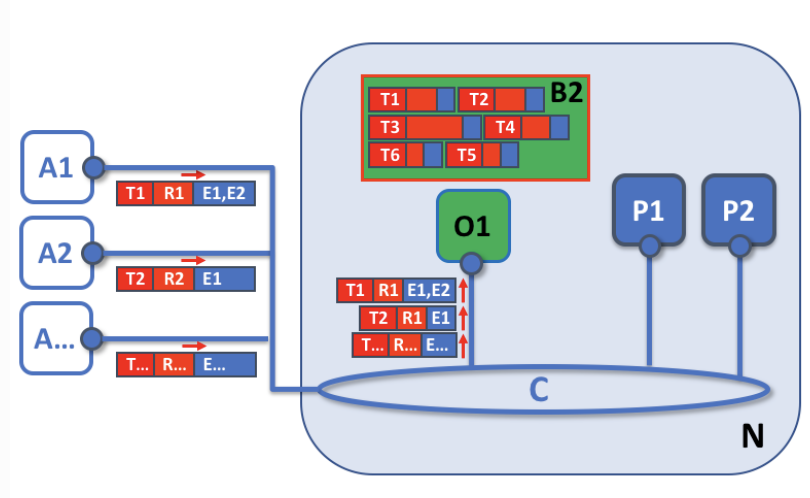
\includegraphics[scale=.5]{start_02}
			\centering
		\end{figure}
	\url{https://hyperledger-fabric.readthedocs.io/en/release-2.0/orderer/ordering_service.html}
	\end{frame}

	\begin{frame}
		\frametitle{Contexto}
		Cada una de las organizaciones tiene su propia Autoridad Certificadora CA.
		\begin{figure}[h]
			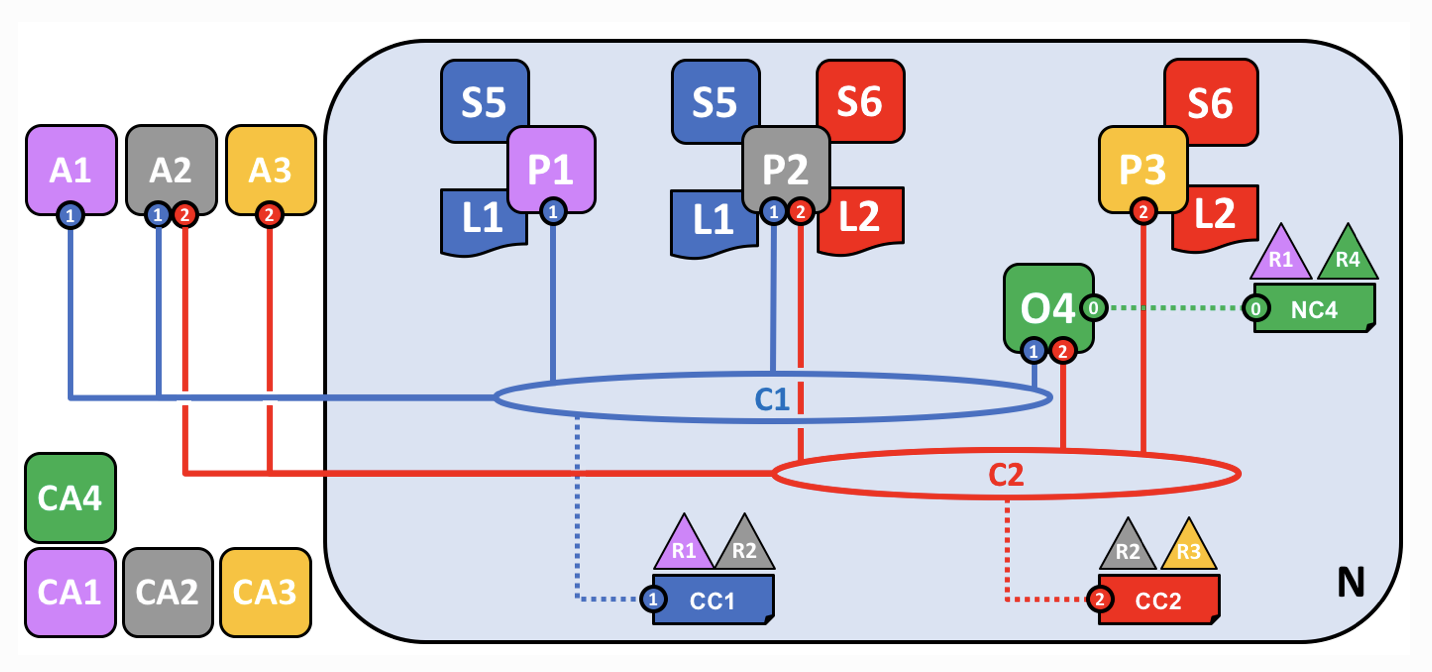
\includegraphics[scale=.3]{start_01}
			\centering
		\end{figure}
	\end{frame}
	
	\begin{frame}
		\frametitle{Contexto}
		\begin{figure}[h]
			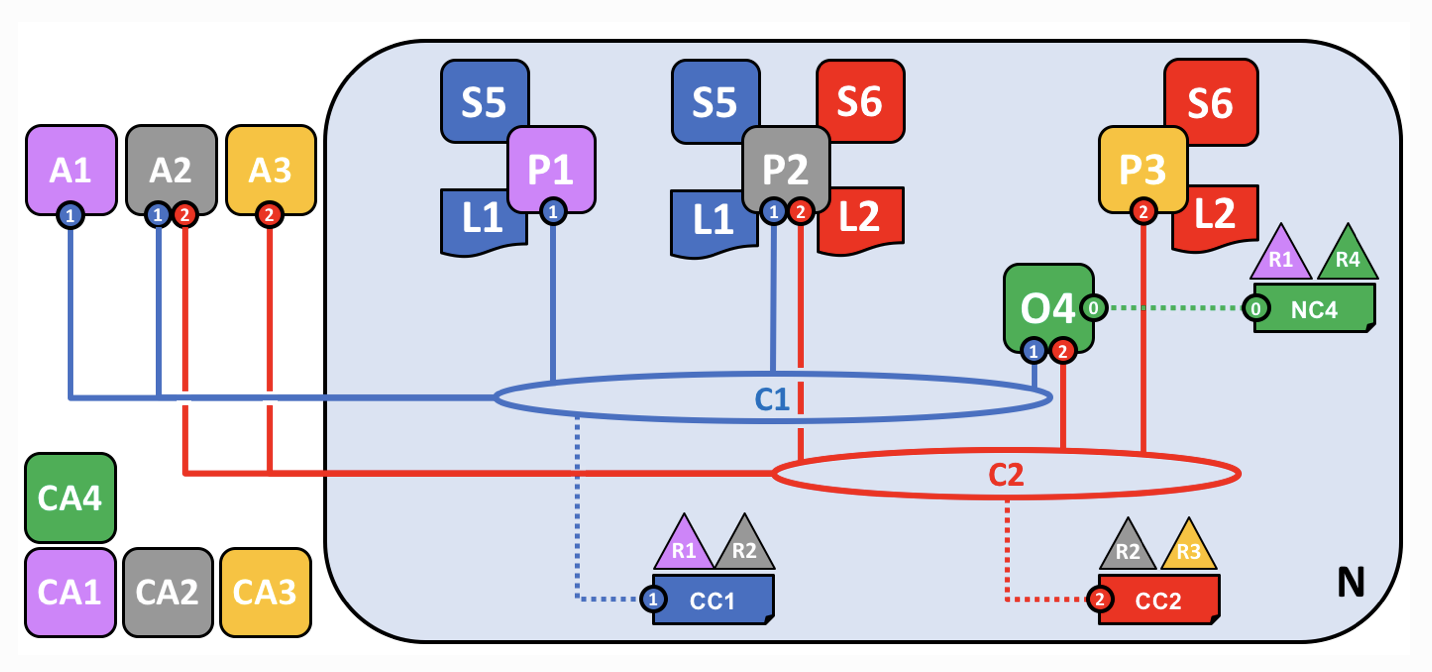
\includegraphics[scale=.4]{start_01}
			\centering
		\end{figure}
		\url{https://hyperledger-fabric.readthedocs.io/en/release-2.0/network/network.html}
	\end{frame}
	
	\subsection{Ejecución}
	
	\begin{frame}
		\frametitle{Ejecución}
		Una vez descargado Hyperledger Fabric ya es posible interactuar con alguno de los proyectos.\\
		\vspace{4mm}
		En realidad, se descargaron imágenes y ejemplos Docker, esto es, contenedores con aplicaciones precargadas, las cuales se guardaron en la carpeta \textbf{fabric-samples}.
	\end{frame}

	\begin{frame}
		\frametitle{Ejecución}
		Vamos a trabajar con el proyecto test-network que está dentro de la carpeta fabric-samples (cd fabric-samples/test-network).\\
		\vspace{4mm}
		En esa carpeta se encuentra el script \textit{network.sh}, el cual levanta una red Fabric utilizando las imágenes Docker descargadas. Para ver el texto de ayuda del script se puede ejecutar \textit{network.sh -h}
	\end{frame}
	
	\begin{frame}
		\begin{figure}[h]
			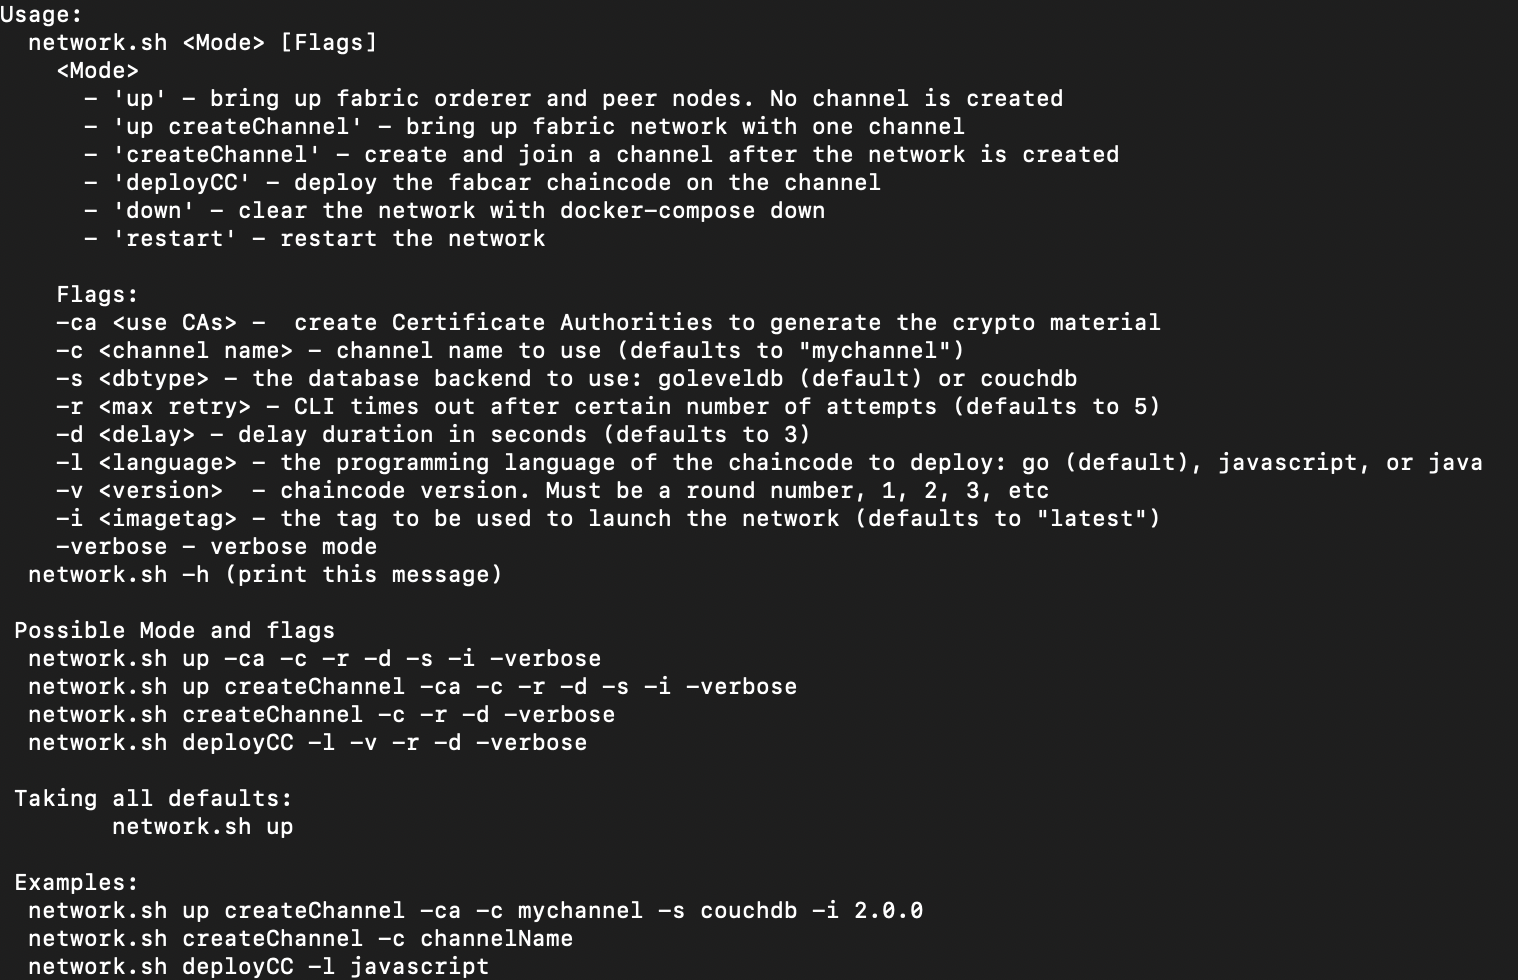
\includegraphics[scale=.4]{start_05}
			\centering
		\end{figure}
	\end{frame}
	
	\begin{frame}
		\frametitle{Crear la red}
		El siguiente comando levanta la red del proyecto \textbf{test-network}, la cual consiste en dos peer nodes y un nodo ordering service; todavía no se crea algún canal:
		\begin{center}
			\setlength{\fboxrule}{1mm}
			\setlength{\fboxsep}{3mm}
			\framebox[9cm][c]{
				\textbf{./network.sh up}
			}
		\end{center}
	\end{frame}
	
	\begin{frame}
		\frametitle{Listar contenedores}
		En este momento se encuentran los contenedores Docker corriendo (los dos nodos y el nodo orden de servicio). El siguiente comando permite listar los contenedores en ejecución:
		\begin{center}
			\setlength{\fboxrule}{1mm}
			\setlength{\fboxsep}{3mm}
			\framebox[9cm][c]{
				\textbf{docker ps -a}
			}
		\end{center}
	\end{frame}
	
	\begin{frame}
		\frametitle{Consorcio}
		\textbf{test-network} tiene  un consorcio (grupo de organizaciones)  con dos miembros Org1 y Org2, además de una organización que mantiene el orden de servicio (ordering service) en la red.\\
		\vspace{4mm}
		Los \textbf{peers nodes} son los componentes fundamentales en cualquier red Fabric. Ellos son los encargados de \textbf{almacenar} en el ledger de la \textbf{blockchain} y validar las transacciones antes de que se suban al ledger. Además, ellos \textbf{ejecutan los smart contracts} que son los que contienen la lógica del negocio.
	\end{frame}
	
	\begin{frame}
		\frametitle{Ordering service}
		Todas las redes Fabric deben incluir un nodo \textbf{ordering service}. Este nodo es el que decide el orden de las transacciones y las transacciones que se incluyen en un bloque.\\
		\vspace{4mm}
		Los \textbf{ordering nodes} hace uso de la configuración de la red (define las capacidades de la red) y los parámetros de configuración del canal. Por defecto, \textbf{ordering nodes} utilizan el algoritmo de consenso \textbf{Raft} (\url{https://raft.github.io}).
	\end{frame}
	
	\begin{frame}
		\frametitle{Canales}
		Actualmente, la red que está se está ejecutando cuenta con 2 peer nodes uno por cada organización (Org1 y Org2) y un ordering node. Ahora vamos a crear un \textbf{canal para las transacciones} entre el consorcio.\\
		\vspace{4mm}
		Recordemos que los canales son \textbf{enlaces privados de comunicación} entre miembros específicos de la red y cada canal tiene su propio ledger de la blockchain.
	\end{frame}
	
	\begin{frame}
		\frametitle{Crear canal}
		Para \textbf{crear un canal} entre las organizaciones Org1 y Org2 y unir los peer nodes al canal se debe ejecutar el siguiente comando:
		\begin{center}
			\setlength{\fboxrule}{1mm}
			\setlength{\fboxsep}{3mm}
			\framebox[9cm][c]{
				\textbf{./network.sh createChannel [-c channel1]}
			}
		\end{center}
	\end{frame}

	\begin{frame}
		\frametitle{Smart contract}
		Para asegurar que una transacción creada a partir de un \textbf{smart contract} sea válida, ésta debe estar firmada por múltiples organizaciones.\\
		\vspace{4mm}
		En Fabric los smart contracts se despliegan en paquetes referidos como \textbf{chaincode}. El chaincode se \textbf{instala} en los peer nodes de la organización y después se \textbf{despliega} en el canal donde se ocupará. Los miembros del canal deben estar de acuerdo con su definición.
	\end{frame}

	\begin{frame}
		\frametitle{Iniciar chaincode}
		Para \textbf{crear un chaincode} en el canal desplegado se debe ejecutar el siguiente comando:
		\begin{center}
			\setlength{\fboxrule}{1mm}
			\setlength{\fboxsep}{3mm}
			\framebox[9cm][c]{
				\textbf{./network.sh deployCC}
			}
		\end{center}
		\textbf{deployCC} instala la chaincode de fabcar en peer0.org1.example.com y peer0.org2.example.com
	\end{frame}
	
	\begin{frame}
		\frametitle{Crear nodo}
		Se puede usar un \textbf{peer node CLI} para \textbf{interactuar con la red} (invocar smart contracts, actualizar canales, instalar y desplegar smart contracts).\\
		\vspace{4mm}
		Los \textbf{binarios de peer} están en la carpeta bin de fabric-samples, la cual \textbf{ya está en el PATH}. También se requiere poner en el PATH la variable FABRIC\_CFG\_PATH:
		\begin{table}[h]
			\centering
			\resizebox{1\textwidth}{!} {
				\begin{tabular}{ | l | }
					\hline
					export FABRIC\_CFG\_PATH=\$PWD/../config/\\
					\hline
				\end{tabular}
			}
		\end{table}
	\end{frame}
	
	\begin{frame}
		\frametitle{Crear nodo}
		Hay que establecer las \textbf{variables de entorno para Org1}, para que CLI pueda operar con ella:\\
		\begin{table}[h]
			\centering
			\resizebox{1\textwidth}{!} {
				\begin{tabular}{ | l | }
					\hline
					Variables de entorno para Org1\\
					\hline
					export CORE\_PEER\_TLS\_ENABLED=true\\
					export CORE\_PEER\_LOCALMSPID=``Org1MSP"\\
					export CORE\_PEER\_TLS\_ROOTCERT\_FILE=\${PWD}/organizations/peerOrganizations/org1.example.com/peers/peer0.org1.example.com/tls/ca.crt\\
					export CORE\_PEER\_MSPCONFIGPATH=\${PWD}/organizations/peerOrganizations/org1.example.com/users/Admin@org1.example.com/msp\\
					export CORE\_PEER\_ADDRESS=localhost:7051\\
					\hline
				\end{tabular}
			}
		\end{table}
	\end{frame}

	\begin{frame}
		\frametitle{Interactuar con la red}
		El nodo \textbf{CLI} puede \textbf{solicitar el ledger} del canal al que pertenece y hacer transacciones: \textbf{Consultar todos los carros}\\
		\begin{table}[h]
			\centering
			\resizebox{1\textwidth}{!} {
				\begin{tabular}{ | l | }
					\hline
					peer chaincode query -C mychannel -n fabcar -c '{``Args":[``queryAllCars"]}'\\
					\hline
				\end{tabular}
			}
		\end{table}
	\end{frame}
	
	\begin{frame}
		\frametitle{Interactuar con la red}
		El nodo \textbf{CLI} puede \textbf{solicitar el ledger} del canal al que pertenece y hacer transacciones: \textbf{Cambiar dueño de un auto}\\
		\begin{table}[h]
			\centering
			\resizebox{1\textwidth}{!} {
				\begin{tabular}{ | l | }
					\hline
					peer chaincode invoke -o localhost:7050 --ordererTLSHostnameOverride\\
					orderer.example.com --tls true --cafile\\
					\${PWD}/organizations/ordererOrganizations/example.com/orderers/orderer.example.com/msp/tlscacerts/tlsca.example.com-cert.pem\\
					-C mychannel -n fabcar --peerAddresses localhost:7051 --tlsRootCertFiles\\
					\${PWD}/organizations/peerOrganizations/org1.example.com/peers/peer0.org1.example.com/tls/ca.crt\\
					--peerAddresses localhost:9051 --tlsRootCertFiles\\ \${PWD}/organizations/peerOrganizations/org2.example.com/peers/peer0.org2.example.com/tls/ca.crt\\
					-c '{``function":``changeCarOwner",``Args":[``CAR9",``Dave"]}'\\
					\hline
				\end{tabular}
			}
		\end{table}
	\end{frame}
	
	\begin{frame}
		\frametitle{Interactuar con la red}
		Debido a que la política de la red requiere que Org1 y Org2 aprueben la transacción, el \textbf{chaincode invoca} a ambos \textbf{peers} utilizando un \textbf{certificado TLS}.\\
		\vspace{4mm}
		El \textbf{chaincode} se instala en los \textbf{peer nodes} de la organización y \textbf{después se despliega} en el canal donde se ocupará. Los miembros del canal deben estar de acuerdo con su definición.
	\end{frame}
	
	\begin{frame}
		\frametitle{Validar cambios}
		Ahora, se pueden \textbf{validar los cambios} en el ledger de la blockchain. En esta ocasión se va a utilizar el nodo \textbf{peer de Org2}, para ello hay que exportar las variables de entorno de Org2:\\
		\begin{table}[h]
			\centering
			\resizebox{1\textwidth}{!} {
				\begin{tabular}{ | l | }
					\hline
					Variables de entorno para Org2\\
					\hline
					export CORE\_PEER\_TLS\_ENABLED=true\\
					export CORE\_PEER\_LOCALMSPID=``Org2MSP"\\
					export CORE\_PEER\_TLS\_ROOTCERT\_FILE=\${PWD}/organizations/peerOrganizations/org2.example.com/peers/peer0.org2.example.com/tls/ca.crt\\
					export CORE\_PEER\_MSPCONFIGPATH=\${PWD}/organizations/peerOrganizations/org2.example.com/users/Admin@org2.example.com/msp\\
					export CORE\_PEER\_ADDRESS=localhost:9051\\
					\hline
				\end{tabular}
			}
		\end{table}
	\end{frame}

	\begin{frame}
		\frametitle{Validar cambios}
		El nodo \textbf{CLI} puede \textbf{solicitar el ledger} del canal al que pertenece y hacer transacciones: \textbf{Consultar un carro}\\
		\begin{table}[h]
			\centering
			\resizebox{1\textwidth}{!} {
				\begin{tabular}{ | l | }
					\hline
					peer chaincode query -C mychannel -n fabcar -c '{``Args":[``queryCar",``CAR9"]}'\\
					\hline
				\end{tabular}
			}
		\end{table}
	\end{frame}

	\begin{frame}
		\frametitle{Dar de baja la red}
		Para \textbf{terminar} un proyecto se debe \textbf{dar de baja la red}. El comando \textbf{down} detiene y elimina los nodos, los contendores, las organizaciones, el material criptográfico, los chaincodes, los registros Docker, los canales y los volúmenes Docker previamente ejecutados.
		\begin{center}
			\setlength{\fboxrule}{1mm}
			\setlength{\fboxsep}{3mm}
			\framebox[9cm][c]{
				\textbf{./network.sh down}
			}
		\end{center}
	\end{frame}
	
	\subsection{Logspout}
	
	\begin{frame}
		\frametitle{Logspout (monitordocker.sh)}
		Es una \textbf{bitácora} de cualquier evento en la red, esta herramienta \textbf{recolecta cualquier flujo de salida} de diferentes contenedores. El script está en commercial-paper/organization/digibank/configuration/cli/. Para \textbf{iniciar} el monitor:\\
		\begin{center}
			\begin{tabulary}{\linewidth}{L}
				\hline
				./monitordocker.sh net\_test \\
				\hline
			\end{tabulary} 
		\end{center}
		Para \textbf{detener} el monitor:
		\begin{center}
			\begin{tabulary}{\linewidth}{L}
				\hline
				docker stop logspout \\
				\hline 
				docker rm logspout \\
				\hline
			\end{tabulary} 
		\end{center}
	\end{frame}
	
	\section{Referencias}
	
	\begin{frame} [allowframebreaks]
		\frametitle{Referencias}
		\nocite{hyper, docker}
		\bibliographystyle{plain}
		\bibliography{biblio}
	\end{frame}
\end{document}